\input{configuration.src}

\addbibresource{./bibliography-collection/lithie.bib}

\title{Trusting Trust Revisited}
\subtitle{Preventing Software Supply Chain Attacks\hfill\\Using Modern Methods}
\institute{Institute of Distributed Systems, Ulm University}
\tag{Seminar}

\author{Florian Sihler}
\email{florian.sihler@uni-ulm.de}
\outro{Ulm, \today}
\license[]{\url{https://creativecommons.org/licenses/by-sa/4.0/}\quad\ccbysa}
% \href{https://creativecommons.org/licenses/by-sa/4.0/}{\ccbysa}
\date{February 12, 2021}

\begin{document}

\section{Motivation}

\begin{frame}{\space}
    \pause{}\begin{layout-imageonly}
    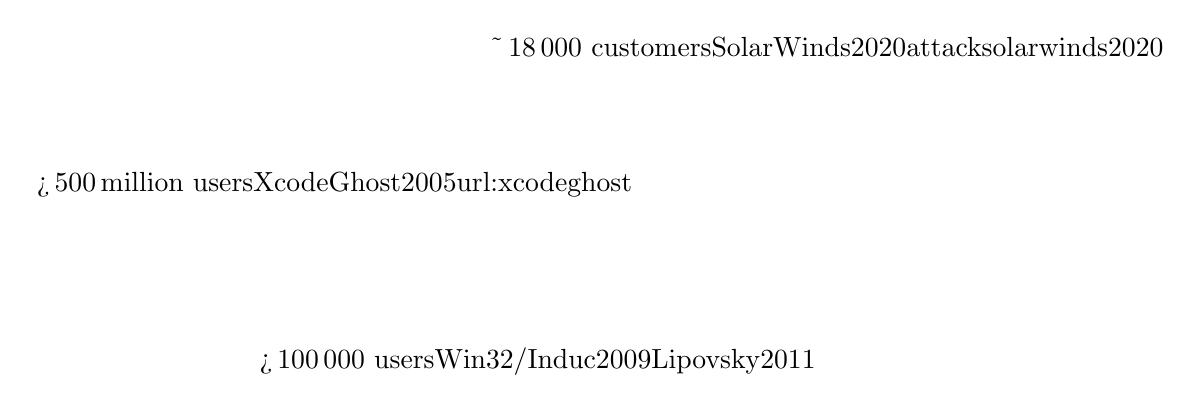
\begin{tikzpicture}
        \node at(0.75,0.25) {\typesetBox{>\,500\,million users}{XcodeGhost}{2005}{url:xcodeghost}};
        \node at(7,2) {\typesetBox{\textasciitilde\,18\,000 customers}{SolarWinds}{2020}{attacksolarwinds2020}};
        \node at(3.33,-2) {\typesetBox{>\,100\,000 users}{Win32/Induc}{2009}{Lipovsky2011}};
    \end{tikzpicture}
\end{layout-imageonly}
\note{\textbf{X Minuten}}
\note[itemize]{
    \item Angriffsmuster Rede von Ken Thompson
    \item >500 mio XcodeGhost
    \item 18\,000 Kunden Solar Winds, auch US-Regierung
    \item 100\,000de Nutzer bei Win32/Induc (Delphi)
}
\end{frame}

\def\tblockfont#1{#1}
\tblocksize=0.95cm
\def\boostrapping{%
\begin{t-diagram}[tborder/.append style={draw=none,fill=lgray,rounded corners=4pt}]
    \begin{scope}[tborder/.append style={fill=hl-shade}]
        \onslide<2->{\tblock[g]{\tblocksize*8+4*\tblockoffset,2*\tblocksize+2*\tblockoffset}{\SL{}}{\ML{}}{\ML{}}}
    \end{scope}
    \begin{scope}[tborder/.append style={densely dashed}]
    \onslide<3->{\tblock[b]{2*\tblocksize+\tblockoffset,-\tblocksize-\tblockoffset}{T}{\ML{}}{\ML{}}}
        \onslide<5->{\tblock[c]{\tblocksize*4+\tblockoffset*2,0}{\SL0}{\ML{}}{\ML{}}}
        \onslide<7->{\tblock[f]{\tblocksize*6+3*\tblockoffset,\tblocksize+\tblockoffset}{\SL1}{\ML{}}{\ML{}}}
    \end{scope}
    \onslide<4->{\tblock[a]{0,0}{\SL0}{\ML{}}{T}}
    \onslide<6->{\tblock[d]{\tblocksize*2+\tblockoffset,\tblocksize+\tblockoffset}{\SL1}{\ML{}}{\SL0}}
    \onslide<8->{\tblock[e]{\tblocksize*4+2*\tblockoffset,2*\tblocksize+2*\tblockoffset}{\SL{}}{\ML{}}{\SL1}}
\end{t-diagram}
}

\section{The Attack}
\SidebarCite{book:mckeemanCompilerGenerator}
\SidebarCite{Thompson1984}
\def\disableos{\def\onslide<##1>##2{##2}}
\newsavebox\bootstrapbox
\savebox\bootstrapbox{\disableos\boostrapping}

\def\infectingdc{%
\onslide<12->{\node[bc] (0) at (0,1.4) {\faFileText};}
\onslide<13->{
    \node[bc=lgray] (1) at (0,0) {\faFile\llap{\color{lgray}\tiny\faCogs\;}};
    \draw[tarrow=hl-shade] (0) -- (1);
}
\onslide<14->{
    \node[bc] (2) at (2,0) {\cfl{hl-shade}};
    \draw[tarrow=hl-shade] (1) -- (2);
}
\onslide<15->{
    \node[bc=lgray] (3) at (2,1.4) {\faFileText};
    \draw[tarrow=lgray] (3) -- (2);
}

\onslide<16->{
    \node[bc] (4) at (4,0) {\cfl{hl-shade}};
    \draw[tarrow=hl-shade] (2) -- (4);
}
% \node[bc] (2) at (4,0) {\cfl{hl-shade}}};
}

\makeatletter
\begin{frame}[fragile]{The Attack}
\begin{layout-imageonly}
    \only<1-8|handout:0>{\begin{center}\scalebox{0.9}{\boostrapping}\end{center}}
    \only<9->{
\begin{tikzpicture}
    \node[scale=0.6,right] (bootstrap) at (0,0) {\usebox{\bootstrapbox}};
\begin{scope}[shift=(bootstrap.east),xshift=1.85cm,yshift=-0.69cm]
    \infectingdc
\end{scope}
    \node at(0,-3.5) {};
\end{tikzpicture}}%
\begin{onlyenv}<9->
\strut~\vspace*{-7em}\\
\hspace*{.265\linewidth}\begin{minipage}[b]{0.75\linewidth}
\lstfs{8}\begin{plaincpp}[morekeywords={[1]{if,contains}},morekeywords={[4]{source}}]
!*\onslide<11->*!inject = 'inject = %c%s%c;
if source contains "compile()":
  prepend("compile()", inject % 34, inject, 34)'

if source contains "compile()":
  prepend("compile()", inject % 34, inject, 34)

!*\onslide<10->*!compile();
\end{plaincpp}
% !*\onslide<10->*!if source contains "if(check(pw))":
% !*\onslide<10->*!  replace(line, "check", "\"a\" == ");
\end{minipage}%
\end{onlyenv}% fake slidecounter thinking max
\only<9-10>{}%
\end{layout-imageonly}
\note{\textbf{Y Minuten}}
\note[itemize]{
    \item Zuerst: Bootstrapping (Go-Compiler seit 1.5)
    \item Wir vereinfachen einmal mit 'compile'
    \item Einbau von Quine
    \item Einfügen des immer selben Codes (lässts ich erweitern)
    \item Infiziert nachfolger
}
\end{frame}
\SidebarReset

\def\ddc{%
\onslide<6->{\node[bc] (0) at (0,1.4) {\faFileText};
\node[left=0.5cm,darkgray] at(0.west) {1.}; \tagS{0}{A}}
\onslide<7->{\node[bc] (1) at (2,1.4) {\!\faCogs};
\draw[tarrow=lgray] (0) -- (1);}
\onslide<8->{\node[bc] (2) at (4,1.4) {\cfl{lgray}};
\draw[tarrow=lgray] (1) -- (2);}
%\begin{pgfonlayer}{background}
    \onslide<9->{\draw[btdl@color@primary,ultra thick,line cap=butt] (1) to[bend left=42,edge node={node[circle,fill=white,inner sep=2pt] {$=$}}] (2);}
%\end{pgfonlayer}
% cheep overlay can't use background as this fails background onslide overwrite
\onslide<7->{\tagN{1}{A}}

\onslide<10->{\node[bc] (3) at (0,0) {\faFileText};
\tagS{3}{A}
\node[left=0.5cm,darkgray] at(3.west) {2.};}
\onslide<11->{\node[bc] (4) at (2,0) {\!\faCogs};
\tagN{4}{B}\draw[tarrow=lgray] (3) -- (4);}
\onslide<12->{\node[bc] (5) at (2,-1.4) {\cfl{lgray}};
\tagS{5}{A}
\draw[tarrow=lgray] (4) -- (5);}

\onslide<13->{\node[bc] (6) at (0,-1.4) {\faFileText};
\tagS{6}{A}
\draw[tarrow=lgray] (6) -- (5);}

\onslide<14->{\node[bc] (7) at (4,-1.4) {\cfl{lgray}};
\draw[tarrow=lgray] (5) -- (7);}

%\begin{pgfonlayer}{background}
    \onslide<15->{\draw[btdl@color@primary,ultra thick,line cap=butt] (2) to[bend left=42,edge node={node[circle,fill=white,inner sep=2pt] {$=$}}] (7);}
%\end{pgfonlayer}

\onslide<8->{\node[bc] (c2) at (4,1.4) {\cfl{lgray}};\tagS{2}{A}}
\onslide<14->{\node[bc] (c7) at (4,-1.4) {\cfl{lgray}};
\tagS{7}{A}}
}


\section{Diverse Double Compiling}
% \SidebarCite{pdf:ddc}
\nocite{pdf:ddc}
\begin{frame}{Diverse Double Compiling}
    \begin{layout-imageonly}
        \centering\begin{tikzpicture}[bc/.default={lgray}]
            \onslide<2->{\node[bc] (0) at (0,1.4) {\faFileText};}
            \onslide<3->{\node[bc] (1) at (-1.25,0) {\!\faLaptop};
            \node[bc] (2) at ( 0,0) {\!\faLaptop};
            \node[bc] (3) at ( 1.25,0) {\!\faLaptop};

            \draw[tarrow=lgray] (0) -- (1);
            \draw[tarrow=lgray] (0) -- (2);
            \draw[tarrow=lgray] (0) -- (3);}

            \onslide<4->{\node[bc=lgray] (a1) at (-1.25,-1.4) {\cfl{lgray}};
            \node[bc=lgray] (a2) at ( 0,-1.4) {\cfl{lgray}};
            \node[bc=lgray] (a3) at ( 1.25,-1.4) {\cfl{lgray}};

            \draw[tarrow=lgray] (1) -- (a1);
            \draw[tarrow=lgray] (2) -- (a2);
            \draw[tarrow=lgray] (3) -- (a3);}

            \onslide<5->{\path (a1) -- (a2) node[btdl@color@primary,pos=0.5] {$=$};
            \path (a2) -- (a3) node[btdl@color@primary,pos=0.5] {$=$};}
            \onslide<2->{\node[below=.15cm] at (current bounding box.south) {Reproducible};}

            \begin{scope}[xshift=5.5cm]
                \ddc
            \end{scope}

        \end{tikzpicture}
    \end{layout-imageonly}
\end{frame}
% \SidebarReset

\section{CHAINIAC}
\def\chainc{%
\onslide<4->{\node[br=hl-shade] (r) at (0.25,0) {\sbfamily Release\nodepart{two}\smaller\faKey~~\faKey~~\faKey~~\faKey};}
\foreach \a in {45,15,-15,-45} {
    \onslide<3->{\node[bc] (d\a) at(\a+180:1.66cm) {\!\faLaptop};}
    \onslide<4->{\draw[tarrow=lgray] (d\a) -- (r);}
}
\begin{scope}[xshift=4cm]
    \onslide<5->{\node[bc] (s0) at (d-45-|-1.33,1) {\faBuilding};
    \node[bc] (s1) at (-1.33,0) {\faBuilding};
    \node[bc] (s2) at (d45-|-1.33,1) {\faBuilding};}

    \onslide<6->{\node[bc=hl-shade] (s) at (0,0) {\faKey};
    % \node[circle,minimum width=2*1.66cm] (sc) at (0,0) {};
    \foreach \i in {0,1,2} {
        \draw[tarrow=lgray] (s\i) -- (s);
    }}
\end{scope}

\begin{scope}[xshift=6.15cm,yshift=.75cm]
    \begin{pgfinterruptboundingbox}
    \foreach \i/\a/\o in {0/7/8,1/6/7,2/5/7,3/4/7} {%
        \def\c{lgray}%
        \ifnum\i=0\def\c{hl-shade}\fi%
        \onslide<\o->{\node[bc=\c,text width=.25em] (t\i) at (0,-\i/2) {};}
        %\node[darkgray,scale=0.75] at (t\i) {\a};
    }
    \onslide<7->{\node[brs=lgray,text width=.25em,text height=.25em] (tc1) at (0.66,-1/2) {};}
    \onslide<7->{\node[brs=lgray,text width=.25em,text height=.25em] (tc3) at (0.66,-3/2) {};}
    \begin{pgfonlayer}{background}
        \onslide<7->{\draw[tarrow=lgray,line cap=round] (t3)++(0,-.5cm) coordinate (lrc-end) -- ($(t0)+(0,0.75cm)$);}
        \onslide<7->{\draw[t=lgray,line cap=round] (tc1) -- (lrc-end-|tc3) (tc1) -- (t1) (t2) -- (tc3) -- (t3);}
        \onslide<8->{\draw[t=lgray,line cap=round] (t0) -- (tc1);}
    \end{pgfonlayer}
    \end{pgfinterruptboundingbox}
\end{scope}

\begin{scope}[xshift=9.5cm]
    \onslide<9->{\node[bc] (u) at (d-15-|0,0) {\faRefresh};
    \foreach[count=\i] \x/\y in {0/0,-.75/0,.75/0,-.375/-.5,.375/-.5} {
        \node[darkgray,scale=0.9] (u\i) at(\x,\y-.75) {\faUser};
        \draw[t=lgray] (u\i) -- (u);
    }}
\end{scope}

\begin{scope}[yshift=2cm]
\begin{pgfinterruptboundingbox}
    \onslide<2->{\fill[lgray,rounded corners=1.5pt] (-1.66-.7,0) rectangle (9.5+.75+.6,0.1) coordinate (ue); \coordinate (us) at (-1.66-.7,0.1);
    \draw[line width=.5ex,btdl@color@background] (1.66,0) -- ++(0,.1) coordinate (u1);
    \draw[line width=.5ex,btdl@color@background] (5,0) -- ++(0,.1) coordinate (u2);
    \draw[line width=.5ex,btdl@color@background] (8,0) -- ++(0,.1) coordinate (u3);}
    \onslide<4->{\path[darkgray] (us) -- (u1) node[midway,above=-.1cm] {\strut Developers};}
    \onslide<6->{\path[darkgray] (u1) -- (u2) node[midway,above=-.1cm] {\strut Cothority};}
    \onslide<8->{\path[darkgray] (u2) -- (u3) node[midway,above=-.1cm] {\strut Timeline};}
    \onslide<9->{\path[darkgray] (u3) -- (ue) node[midway,above=-.1cm] {\strut Mirror};}
\end{pgfinterruptboundingbox}
\end{scope}
}

\SidebarCite{Nikitin2017}
\begin{frame}{CHAINIAC}
\begin{layout-imageonly}
    % TODO: bei animationen zuerst grayed out und dann einblenden
\centering\vspace*{-.25em}\begin{tikzpicture}[bc/.default={lgray},br/.default={lgray}]
    \chainc
\end{tikzpicture}
\end{layout-imageonly}
\end{frame}
\SidebarReset

\section{Conclusion}
\nocite{url:repbuilds}
\def\conclusionshow{%
\begin{tikzpicture}
    \onslide<2->{\begin{scope}[xscale=0.8,yshift=-.9cm]
        {\disableos\infectingdc}%
    \end{scope}}
    \onslide<3->{\begin{scope}[bc/.default={lgray},xshift=7.25cm,xscale=0.8]
        {\disableos\ddc}%
    \end{scope}}
\end{tikzpicture}}
\begin{frame}{Conclusion}
\begin{layout-imageonly}
    \centering\vfill\only<handout:0|6->{%
        \colorlet{hl-shade}{gray!80!white}%#
        \colorlet{btdl@color@primary}{gray!80!white}%
        \tikzset{every path/.append style={opacity=0.25}}
    }
    \only<1-3>{\hspace*{2em}}
\only<4->{\begin{columns}[t]
\begin{column}[c]{0.325\linewidth}
    \null\vspace*{2em}\vfill\onslide<7->{\faAngleRight~Reproducible Builds\bigskip\par}
    \onslide<8->{\faAngleRight~Tool support\vspace*{4em}\par}
    \onslide<9->{\only<10->{\sbfamily}\faAngleRight~\only<10->{Trusting }Trust\strut}
\end{column}\hfill
\begin{column}{0.6\linewidth}}
    \centering\only<4->{\resizebox{\linewidth}{!}}\conclusionshow\hspace*{5em}\vspace*{3em}\\%
    \only<4->{\onslide<5->{\resizebox{.925\linewidth}{!}{\begin{tikzpicture}[bc/.default={lgray},br/.default={lgray}]
        {\disableos\chainc}
    \end{tikzpicture}}\null}}
    \only<4->{\vspace*{1.25em}\end{column}\end{columns}\hspace*{15em}}\vfill
\end{layout-imageonly}
    % [TODO] Rückblick: Problem. Dann Übersicht: DDC + CHAINIAC + weitere Probleme: eine Option in vielen. \(\Rightarrow\) Rückblende zu warum \enquote{Trust}
\note[itemize]{
    \item Rückblick bisherige Themen: Angriffe, DDC, Chainiac
    \item Reproducible Builds effort: Linux Kernel, (MES) C-Compiler,  ...
    \item Tool Support: Docker, APT+CHAINIAC, diffoscope (Vergleich), RepLoc (Suche)...
    \item Schwachstellen -- sichert \textbf{nicht} den Code sondern nur, dass nichts modifiziert wird.
    \item SolarWinds Breach nach Wheel mit RepBuilds behebbar
    \item Aufwand für einen zu viel... Nicht nur den Herstellern vertrauen, sondern allen...
    \item Nicht nur Trust => Trusting Trust
}
\end{frame}


\pdfbookmark[0]{Endfolie -- Quellen}{endfolie}%
\end{document}
